\section{Results}
\label{sec:results}

\begin{table}[t]
\centering
\caption{Matched-scale regressions (Equation~\ref{eq:group}) behind all claims of Section~\ref{sec:results}. Each row is
one fit (or, for $\Delta$ rows, the interaction of every fixed effect with the bin or network in a pooled fit). Outcomes: score
divided by the split-half reference (all datasets; word-pair bins, both bins by the all-pairs reference); percentile rank of the raw score among the 118 models within each dataset and network (language vs.\ MD,
whose references are too small to divide by). Fits: all datasets, dataset-unit and lineage random intercepts (REML,
Satterthwaite $t$-tests); word-pair bins, one fit over both bins with measure-by-bin, lineage and lineage-by-bin random
intercepts; networks, dataset fixed effects and a lineage random intercept (all REML, Satterthwaite $t$-tests). All datasets with a
robust-$z$ outcome: Table~\ref{tab:summary-z}. Coefficient (SE); reference: Standard LLM of the same size and perplexity. $^{*}p<.05$, $^{**}p<.01$, $^{***}p<.001$.}
\label{tab:summary}
\setlength{\tabcolsep}{3pt}
\resizebox{\linewidth}{!}{%
\begin{tabular}{@{}lcccccc@{}}
\toprule
 & Memory $\beta_M$ & Data $\beta_D$ & $M\times D$ $\beta_{MD}$ & $\log_{10}$ params $\beta_S$ & $\log_{10}$ PPL $\beta_P$ & C-BabyLM vs.\ LLM \\
\midrule
\multicolumn{7}{@{}l}{\textit{All datasets \quad (16 reading measures; 8 neural datasets)}} \\
\quad Behavior & $+.028^{**}$ (.011) & $+.030^{*}$ (.014) & $-.031^{*}$ (.015) & $-.033^{***}$ (.004) & $-.027^{***}$ (.004) & $+.027^{*}$ (.011) \\
\quad Brain & $-.189^{*}$ (.092) & $-.261^{*}$ (.116) & $+.141$ (.136) & $+.201^{***}$ (.054) & $-.183^{**}$ (.061) & $-.309^{**}$ (.111) \\
\addlinespace
\multicolumn{7}{@{}l}{\textit{Syntactic memory load \quad (Natural Stories; Podcast)}} \\
\quad Behavior, easy--easy & $+.006$ (.006) & $+.008$ (.008) & $-.011$ (.008) & $-.004$ (.002) & $+.000$ (.002) & $+.003$ (.006) \\
\quad Behavior, any-hard & $+.018^{**}$ (.006) & $+.027^{**}$ (.008) & $-.032^{***}$ (.008) & $-.028^{***}$ (.002) & $-.006^{*}$ (.002) & $+.013^{*}$ (.006) \\
\quad Behavior, $\Delta$ hard $-$ easy & $+.012$ (.007) & $+.018$ (.009) & $-.021^{*}$ (.010) & $-.023^{***}$ (.003) & $-.006$ (.003) & $+.010$ (.008) \\
\quad Brain, easy--easy & $-.190^{*}$ (.075) & $-.335^{**}$ (.107) & $+.360^{**}$ (.114) & $+.195^{***}$ (.035) & $-.259^{***}$ (.050) & $-.164$ (.085) \\
\quad Brain, any-hard & $-.097$ (.075) & $-.250^{*}$ (.107) & $+.224$ (.114) & $+.146^{***}$ (.035) & $-.291^{***}$ (.050) & $-.123$ (.085) \\
\quad Brain, $\Delta$ hard $-$ easy & $+.092$ (.063) & $+.085$ (.080) & $-.136$ (.094) & $-.049$ (.044) & $-.032$ (.055) & $+.041$ (.082) \\
\addlinespace
\multicolumn{7}{@{}l}{\textit{Word frequency \quad (9 reading measures; Podcast)}} \\
\quad Behavior, frequent--frequent & $+.055$ (.081) & $+.032$ (.105) & $-.042$ (.117) & $-.016$ (.034) & $-.038$ (.028) & $+.046$ (.089) \\
\quad Behavior, any-rare & $+.348^{***}$ (.081) & $+.338^{**}$ (.105) & $-.313^{*}$ (.117) & $-.545^{***}$ (.034) & $-.285^{***}$ (.028) & $+.373^{***}$ (.089) \\
\quad Behavior, $\Delta$ rare $-$ frequent & $+.293^{**}$ (.104) & $+.306^{*}$ (.132) & $-.271$ (.150) & $-.529^{***}$ (.047) & $-.246^{***}$ (.037) & $+.327^{**}$ (.115) \\
\quad Brain, frequent--frequent & $-.126$ (.102) & $-.302^{*}$ (.146) & $+.299$ (.153) & $+.181^{***}$ (.046) & $-.309^{***}$ (.067) & $-.129$ (.113) \\
\quad Brain, any-rare & $-.220^{*}$ (.102) & $-.451^{**}$ (.146) & $+.464^{**}$ (.153) & $+.085$ (.046) & $-.426^{***}$ (.067) & $-.208$ (.113) \\
\quad Brain, $\Delta$ rare $-$ frequent & $-.095$ (.108) & $-.149$ (.138) & $+.165$ (.153) & $-.096$ (.062) & $-.118$ (.084) & $-.079$ (.127) \\
\addlinespace
\multicolumn{7}{@{}l}{\textit{Language vs.\ multiple-demand network \quad (Pereira, Podcast, Tuckute)}} \\
\quad Brain, language & $-.100^{*}$ (.043) & $-.101$ (.058) & $+.093$ (.063) & $+.155^{***}$ (.018) & $-.052^{*}$ (.024) & $-.107^{*}$ (.048) \\
\quad Brain, MD & $-.035$ (.050) & $-.053$ (.063) & $+.065$ (.072) & $+.100^{***}$ (.027) & $-.062$ (.034) & $-.024$ (.060) \\
\quad Brain, $\Delta$ MD $-$ language & $+.086$ (.048) & $+.024$ (.061) & $-.017$ (.073) & $-.043$ (.031) & $+.002$ (.036) & $+.093$ (.061) \\
\bottomrule
\end{tabular}}
\end{table}


\subsection{Constraints are associated with behavioral, not brain, similarity}
\label{sec:results-main}
\label{sec:results-all}

No evaluated model leads on both targets (Figure~\ref{fig:method}B). The Pareto front runs from BabyLM models at the behavioral end (GPTBERT-10M-CausalFocus, .163 of the reference) through Pythia-410M to Standard LLMs at the neural end (Mamba models to Ministral-3-3B, .96). BabyLM models have the highest median behavioral similarity (.141, against .103--.109 for the other groups) and Standard LLMs the highest median brain similarity (.64, against .07--.18).

Group medians confound the constraints with scale. At matched size and perplexity (Table~\ref{tab:summary}, top), both constraints are associated with higher behavioral similarity: memory $+.028$ ($p=.009$) and data $+.030$ ($p=.040$) of the reference. Their interaction is negative ($-.031$), so a model with both constraints gains about as much as a model with one (Constrained-BabyLM vs.\ Standard LLM $+.027$, $p=.019$). Neither constraint is associated with higher brain similarity; both are associated with \emph{lower} brain similarity than Standard LLMs of the same size and perplexity (memory $-.189$, $p=.045$; data $-.261$, $p=.030$; Constrained-BabyLM $-.309$, $p=.007$). Size dissociates the two targets too: at fixed perplexity, larger models are less similar to reading behavior ($-.033$ per decade of parameters, $p<.001$) and more similar to the brain ($+.201$, $p<.001$), whereas lower perplexity raises both.

\paragraph{Robustness.} The two sides of this result differ in robustness. No check yields a brain \emph{advantage} for constrained models, and every check that keeps surprisal as the behavioral predictor keeps the behavioral advantage; the brain \emph{penalty} is less robust (i), so we claim only the absence of a brain advantage. (i) \emph{Training checkpoints} (Appendix~\ref{app:checkpoints}): adding 119 Pythia and BabyLM GPT-2 checkpoints, which fill the perplexity range of the constrained models, keeps the behavioral advantage (memory $+.029$, $p<.01$; data $+.036$; Constrained-BabyLM $+.028$, both $p<.05$) and no brain advantage (memory $-.089$, $p=.34$; data $-.220$, $p=.054$), and so does restricting all models to at most 2B, 1B or 500M parameters. (ii) \emph{No noise reference} (Table~\ref{tab:summary-z}): with robust $z$ scores the behavioral advantage remains (memory $+.29$, data $+.48$ standard deviations, both $p<.05$), and the memory constraint remains associated with lower brain similarity ($-.46$, $p=.041$). (iii) \emph{Same model quantity on both axes} (Appendix~\ref{app:same-predictor}): with surprisal on both axes, constraints are associated with lower brain similarity. With embeddings on both axes, the behavioral data advantage keeps its sign but is not reliable ($p=.052$) and the memory advantage vanishes ($p=.98$): the behavioral advantage is established for surprisal, the standard predictor of reading times, not for the geometry of hidden states. On Natural Stories and Podcast alone (Appendix~\ref{app:two-datasets}), the data constraint is associated with higher behavioral similarity and both constraints with lower brain similarity.

\begin{figure}[t]
\centering
\includegraphics[page=3,trim=0 626 0 0,clip,width=\textwidth]{figures/humanscore_figures.pdf}
\caption{Where could the constraints help? (A) High working-memory load: pairs with at least one DLT-hard word (Natural Stories reading; Podcast ECoG). (B) Rare words: pairs with at least one rare word (Zipf $\leq3$; median over 9 reading measures; Podcast). In A and B, each axis is divided by the all-pairs split-half reference. (C) Multiple-demand network: behavioral similarity as in Figure~\ref{fig:method}B; brain similarity is the mean percentile rank of the raw score on the MD network of Pereira, Podcast and Tuckute. Layout as in Figure~\ref{fig:method}B.}
\label{fig:where}
\end{figure}

\subsection{Syntactically demanding words give only a weak test of the memory constraint}
\label{sec:results-dlt}

If memory-constrained models are more human-like because humans have limited working memory, their advantage should be largest on words that tax it, such as words that close long dependencies \citep{gibson2000dlt}. On pairs containing such a word (Figure~\ref{fig:where}A), the front keeps its shape: small memory-constrained Pile models (Forgetting-Pile-2L and 4L) lead behavior, Standard LLMs lead the brain. At matched scale (Table~\ref{tab:summary}), both constraints are associated with higher behavioral similarity on any-hard pairs (memory $+.018$, $p=.001$; data $+.027$, $p=.002$; Constrained-BabyLM $+.013$, $p=.033$) but not on easy--easy pairs ($+.006$ and $+.008$, both $p=.30$). The bin differences, however, are not reliable (memory $+.012$, $p=.077$; data $+.018$, $p=.057$; Constrained-BabyLM $+.010$, $p=.20$), so we cannot conclude that the advantage is larger where memory load is high. Reading times also carry more model-explainable signal on any-hard pairs (the median model reaches .073 of the all-pairs reference there, against .013 on easy--easy pairs), and the size coefficient is larger there too (difference $-.023$, $p<.001$): on the logarithm of the score, which removes this difference of scale, neither constraint differs between the bins (Appendix~\ref{app:wordclass-dlt}). On the brain side, no constraint is associated with higher similarity in either bin; constrained models are less similar than Standard LLMs on easy--easy pairs (memory $-.190$, $p=.013$; data $-.335$, $p=.003$) and, for the data constraint, on any-hard pairs ($-.250$, $p=.025$).

This is a weak test of the memory constraint. We use Natural Stories because it is the only reading corpus in which DLT-hard words carry a cost beyond length and frequency, and that cost is small: 5.3\,ms (95\% CI $[1.1, 9.5]$), a third of the cost of a rare word in the same corpus (15.5\,ms). The eye-tracking corpora offer no test at all, since there hard words are read as fast as or faster than easy words of the same length and frequency (Appendix~\ref{app:wordclass-dlt}). This agrees with earlier corpus work: in the Dundee eye-tracking corpus, integration cost does not predict reading times on arbitrary words, only on nouns \citep{demberg2008data}, and locality effects in naturalistic reading are mixed overall (reviewed by \citealp{li2027modeling}). Memory limits do shape reading when dependencies are long and controlled, most for readers with low working-memory capacity \citep{li2027modeling}; naturalistic text contains few such dependencies, so neither the memory advantage on any-hard pairs nor the missing bin difference says much about whether a model-side memory limit matches the human one. Rare words, by contrast, slow reading by 15 to 99\,ms in every measure: word frequency is the larger source of difficulty.

\subsection{The behavioral advantage comes from rare words}
\label{sec:results-freq}

Reading times carry most of their model-explainable signal on pairs with a rare word: the median model reaches .92 of the all-pairs reference on any-rare pairs and .22 on frequent--frequent pairs. This is also where the constraint advantage lies (Table~\ref{tab:summary}). On frequent--frequent pairs neither constraint is associated with behavioral similarity (memory $+.055$, $p=.50$; data $+.032$, $p=.76$); on any-rare pairs both are (memory $+.348$, $p<.001$; data $+.338$, $p=.003$; Constrained-BabyLM $+.373$, $p<.001$), and the bin differences are reliable (memory $+.293$, $p=.009$; data $+.306$, $p=.030$; Constrained-BabyLM $+.327$, $p=.007$). The size penalty, too, appears only on rare pairs ($-.545$ against $-.016$). The front (Figure~\ref{fig:where}B), which ranks models by their median over measures, is held by small Standard LLMs (Pythia-70M and OPT-125M at its behavioral end, RWKV4-3B at its neural end). On the brain side the pattern does not carry over: on Podcast, no constraint is associated with higher similarity in either bin, the data constraint is associated with lower similarity in both (frequent $-.302$, $p=.044$; rare $-.451$, $p=.003$) and the memory constraint on rare pairs ($-.220$, $p=.033$), and no bin difference is reliable.

This advantage is defined in units of the human reference, i.e.\ as a share of the reliable reading-time signal. It is not uniform across measures: on rare pairs it comes from GECO and from OneStop first-pass and go-past times, where model scores spread most, and it is reversed in OneStop scan-path time and in ZuCo (Table~\ref{tab:freq-measures}).

\subsection{No advantage on the multiple-demand network}
\label{sec:results-md}

On the neural side, the constraints could help where human working memory is engaged, in the MD network rather than the language network \citep{duncan2010multiple,fedorenko2013broad}. The MD network is hard to predict for every model: raw scores are lower than on the language network in Pereira (median $\Delta\ell$ $.0038$ against $.0059$) and Podcast ($.0022$ against $.0051$), and in Tuckute no model predicts the MD response beyond length and frequency (31--42\% of models score above 0 in each group). Standard LLMs still hold most of the neural end of the front (Figure~\ref{fig:where}C; OPT models up to OPT-66B, joined by the ALiBi model BLOOM-7.1B), and model rankings on the two networks largely agree (Spearman $\rho=.995$ in Pereira, $.80$ in Podcast).

At matched scale (Table~\ref{tab:summary}, bottom), constrained models rank below Standard LLMs on the language network (memory $-.100$, $p=.025$; data $-.101$, $p=.093$; Constrained-BabyLM $-.107$, $p=.028$) and level with them on the MD network (memory $-.035$; data $-.053$; Constrained-BabyLM $-.024$; all $p\geq.40$); the network difference is not reliable (Constrained-BabyLM $+.093$, $p=.13$). No constraint is associated with an advantage on the MD network: constrained models do not match the working-memory network better than standard LLMs.
